\documentclass[a4j,12pt]{jsarticle}
\usepackage{semi}
\begin{document}


\日付{2019/1/15}
\氏名{阿部 希駿}
\タイトル{卒業研究}

\semi

\tableofcontents

\newpage
\section{緒言}
文部科学省が発表した国際学力調査によると世界の中でも日本の学力は上位にある.しかし日本よりも上位の国に比べ.低得点の割合はやや多く,順位を上げるためには低得点層の割合を減らすことが必要である.
低得点層の学生は学習内容の一部がわからないのではなく,「何をしているのかがわからない」「どこがわからないのかもわからない」などという根本的な原因があると推測している.

また各塾の調査では中学,高校で学習する科目の中で数学と英語は苦手になりやすいと言われている\cite{1}.この2科目の共通点である積み上げ型教科という点に注目した.積み上げ型教科とは既に学習した知識を使うことを前提として授業を行う教科である.そのため単元の内容が複雑になるほど必要な前提知識が多くなり,どの単元の内容が使われているかがわかりにくくなる.そのためその単元の内容を理解をすることが難しくなることが問題点としてあげられる.

そこで「学習する単元を前提知識とする単元の概要をあらかじめ説明することで,内容の理解を促進することができる」という仮説を立てた.
この仮説では特に複数の単元の学習内容を用いて学習を行う単元を対象にする.
本研究では,積み上げ型教科の理解力向上を目的として,講義にて学生を対象に実験を行い,この仮説を検証する.

\newpage
\section{教科の特性}
学校で学習する教科には独立型教科と積み上げ型教科に分かれ,それぞれ下図のように積み木のような図で表される.\\

\begin{figure}[H]
\centering
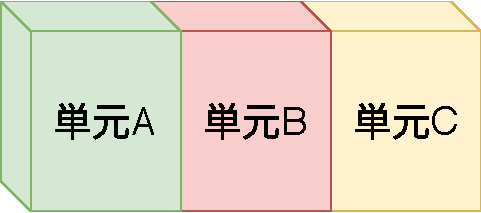
\includegraphics[width=7cm]{02.pdf}
\caption{独立型教科の教育モデル}
\label{fig:02}
\end{figure} 

\begin{figure}[H]
\centering
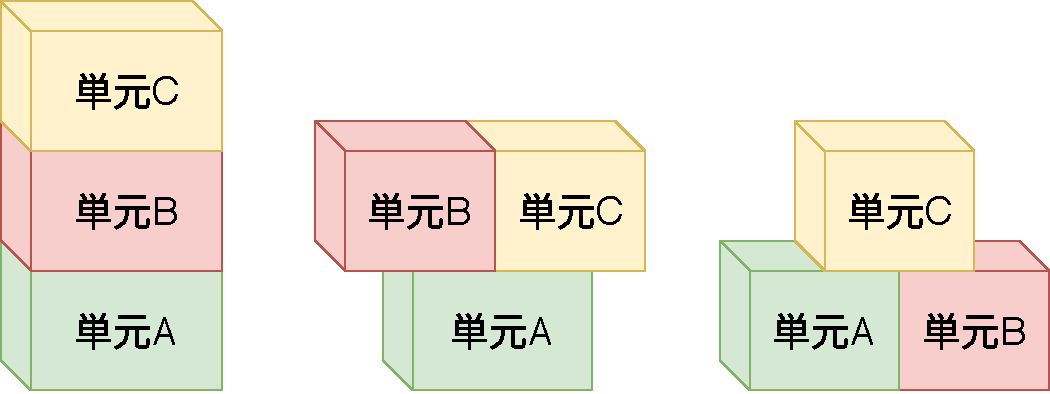
\includegraphics[width=12cm]{03.pdf}
\caption{積み上げ型教科の教育モデル}
\label{fig:03}
\end{figure} 


\subsection{独立型教科}
独立型教科は国語や社会が該当する.
独立型教科では図\ref{fig:01}のように各単元が独立していて関連性があまりないためどの単元から学習しても支障がない.\\
\begin{figure}[H]
\centering
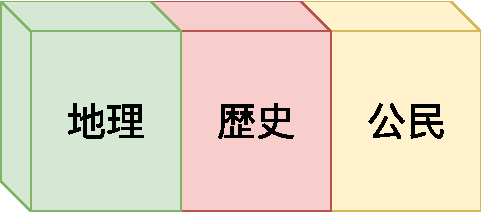
\includegraphics[width=6cm]{01.pdf}
\caption{独立型教科の例}
\label{fig:01}
\end{figure} 

\subsection{積み上げ型教科}
積み上げ型教科では数学や英語が該当する.
積み上げ型教科では図\ref{fig:04}のように学習した内容を次の学習の基礎知識として用いるため,順番に学習していくことになる.\\

\begin{figure}[H]
\centering
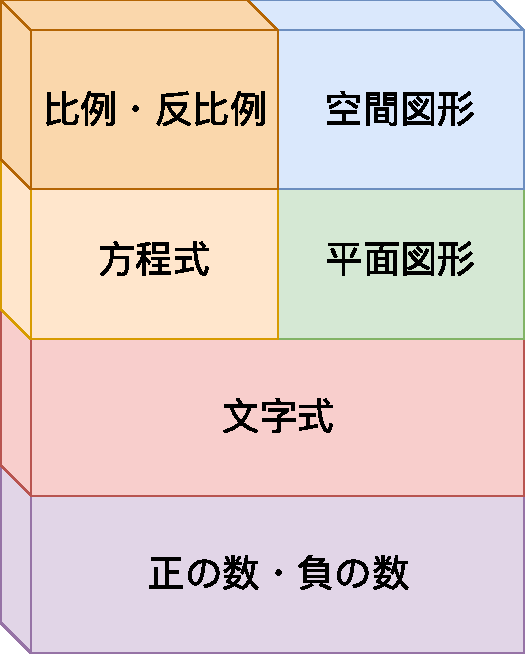
\includegraphics[width=5cm]{04.pdf}
\caption{積み上げ型教科の例}
\label{fig:04}
\end{figure} 

\newpage
\section{ハッシュ関数}

任意のデータを固定長の値であるハッシュ値に置き換えることである.
ハッシュ関数は不可逆的な一方向関数であり,ハッシュ値から元のデータに復元することは不可能である.
ハッシュ値は一定の法則で短縮されているため,違うデータを同じハッシュ値になるように改ざんすることはできない.
そのため改ざんや破損の検知など,ファイルの同一性確認に使用される.
ハッシュ値を元のデータに戻すことはできない.\\

\begin{figure}[H]
\centering
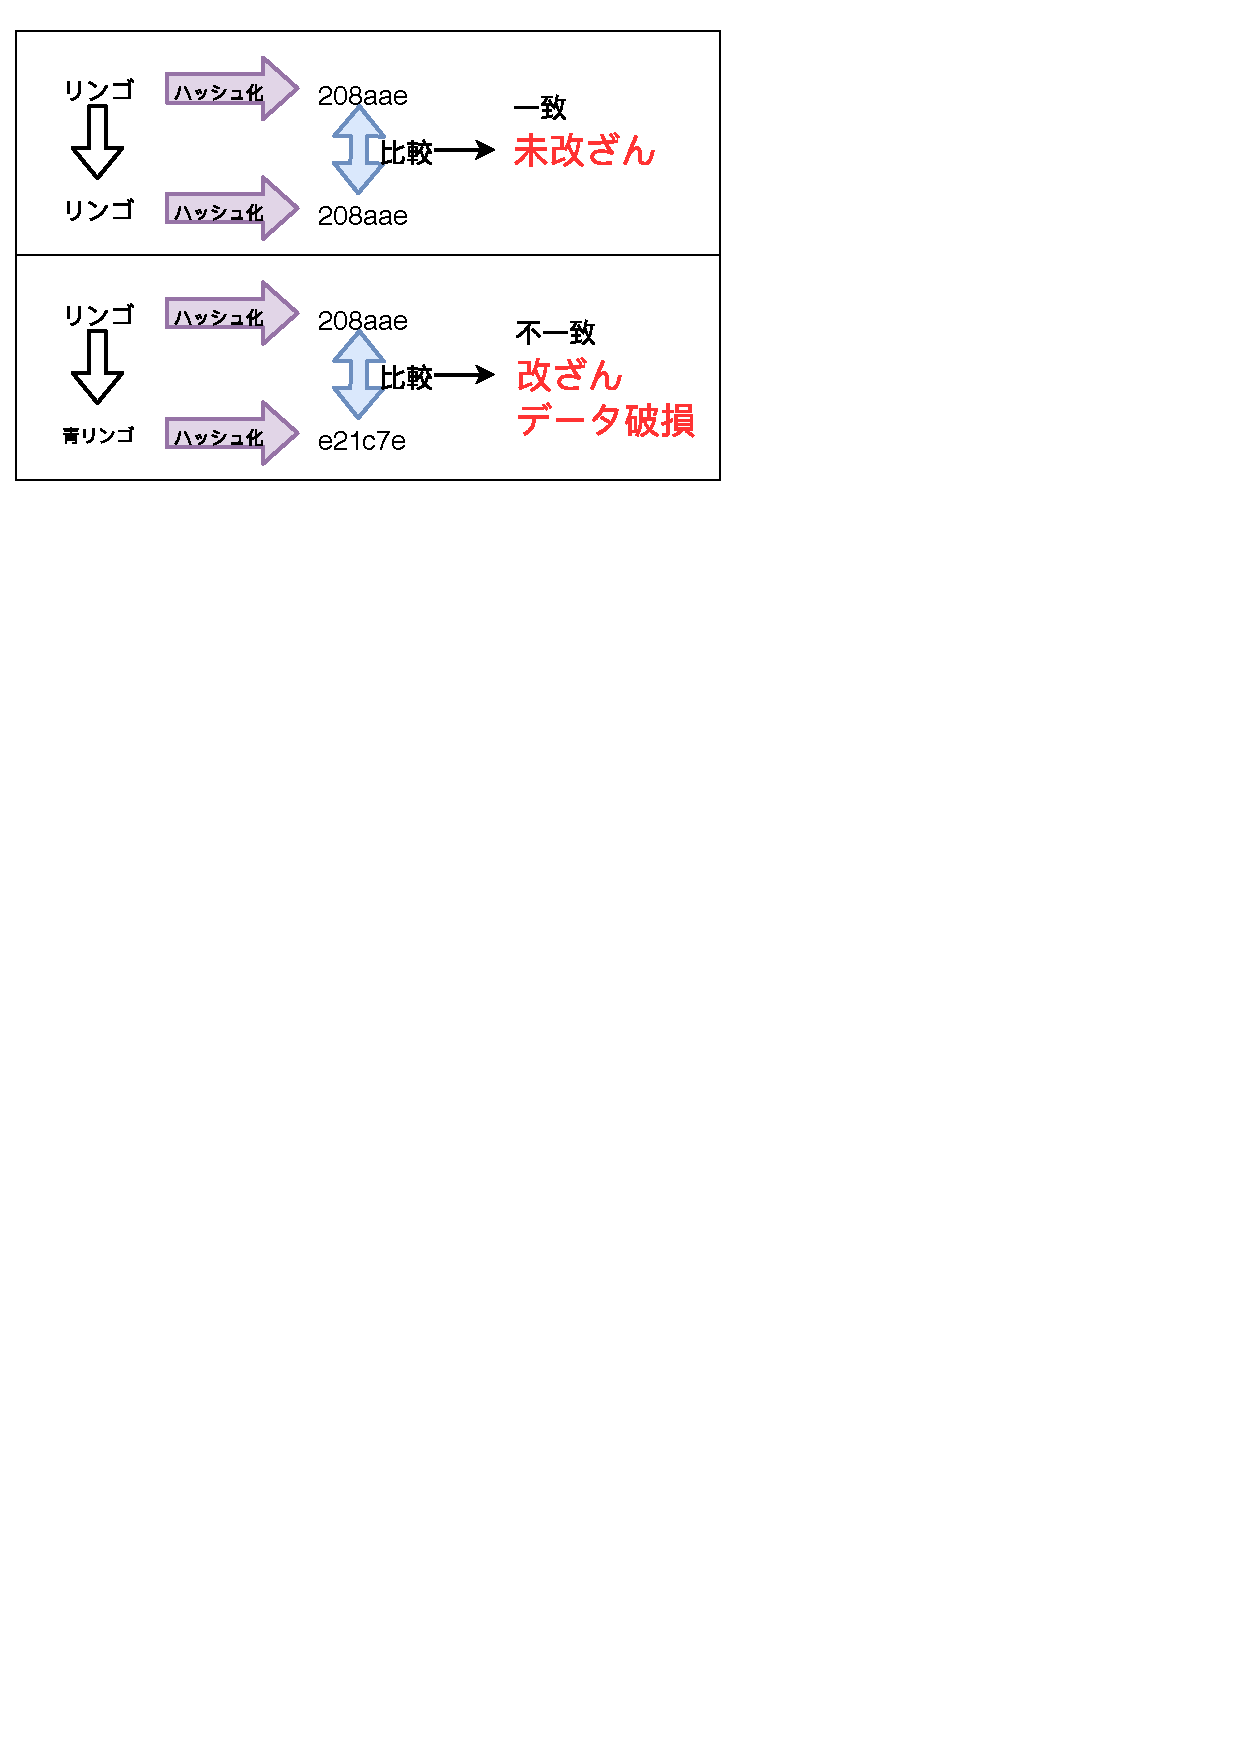
\includegraphics[width=11cm]{hash.pdf}
\caption{ハッシュを用いたファイルの同一性確認の流れ}
\label{fig:no}
\end{figure} 




\section{暗号}
暗号とは通信を行う際,第三者にその内容を知られないようにするための手段である.
元の文に一定の規則を用いて特定の変形を加えることを暗号化,暗号化する前の元の文を平文,暗号から平文に戻すことを復号と呼ぶ.
暗号化する手段が暗号アルゴリズムであり,また暗号化や復号化に使うデータを鍵と呼ぶ.
暗号は特性によって古典暗号と現代暗号に分かれる.
アルゴリズムがわかれば解読が容易になる暗号を古典暗号,アルゴリズムは公開するが鍵を非公開にすれば安全な暗号を現代暗号という.

\newpage
\subsection{共通鍵暗号}
暗号化と復号に同じ鍵を用いる暗号の方式である.
通信相手に鍵を送り,その鍵を用いて情報を暗号化する.
暗号化された情報が送られてきたら,同じ鍵を使って復号する.


\begin{figure}[H]
\centering
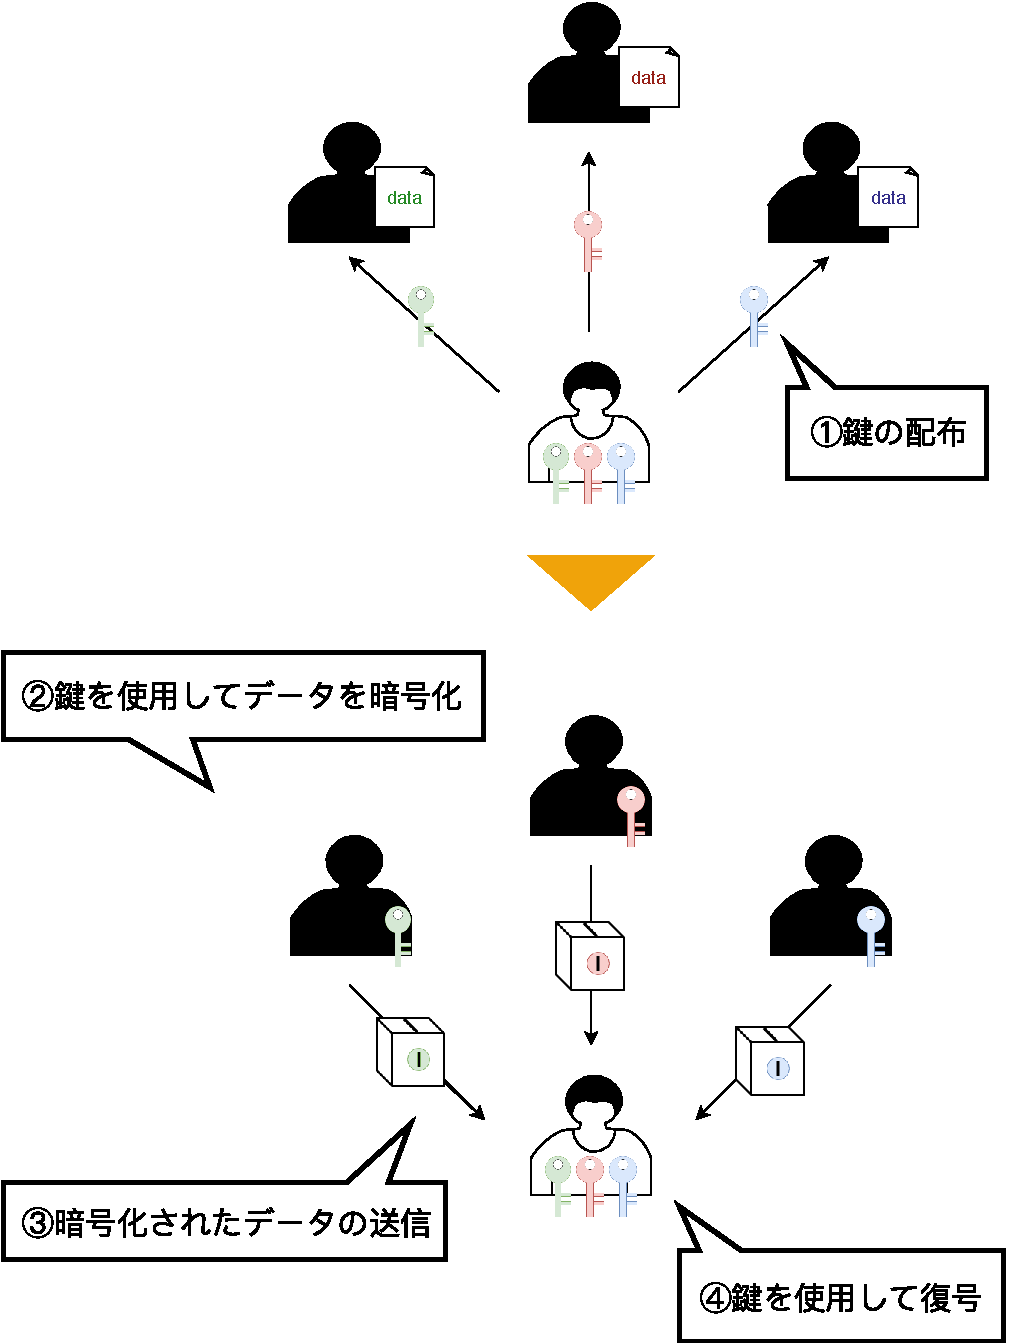
\includegraphics[width=10cm]{kyotu.pdf}
\caption{共通鍵暗号通信の流れ}
\label{fig:no}
\end{figure} 

共通鍵暗号通信では暗号化と同じ鍵を使っているため,鍵を送る際に第三者に傍受される危険がある.
また同じ鍵を複数のユーザーで使用すると,他のユーザーが復号する危険性があるため,ユーザーごとに鍵を生成する必要がある.


\newpage
\subsubsection{換字式暗号の仕組みと例}
平文の文字を他の記号や文字に置き換えて暗号文を作る古典暗号の方式である.
換字式暗号の代表としてシーザー暗号がある.
シーザー暗号は鍵である決められた文字数分のアルファベットをずらして暗号化を行う.
図\ref{fig:05}は鍵が1であるときの例である.\\

\begin{figure}[H]
\centering
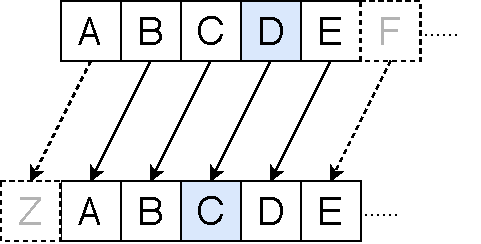
\includegraphics[width=9cm]{05.pdf}
\caption{シーザー暗号の例}
\label{fig:05}
\end{figure} 


\subsubsection{転置式暗号の仕組みと例}
平文の位置を並び替えて暗号文を作る古典暗号の方式である.
転置式暗号の代表としてスキュタレー暗号がある.
スキュタレー暗号はスキュタレーと呼ばれるシリンダーに細長い紙を巻きつけ,平文を横書きに書く.
紙をスキュタレーから外すと順番が入れ替わった暗号ができる.
暗号の受け取る側は同じ半径のスキュタレーを用意し,紙を巻きつけることで復号することができる.
この場合,鍵は同じ直径であることである.\\

\begin{figure}[H]
\centering
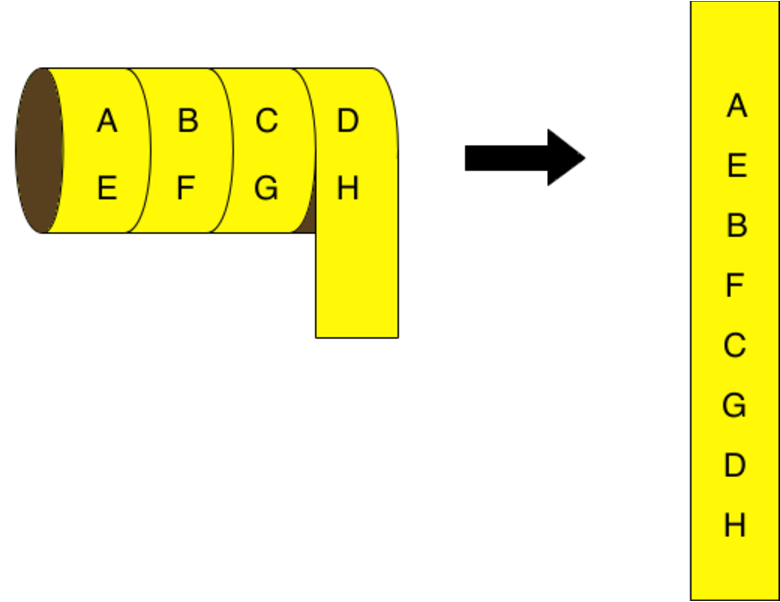
\includegraphics[width=8cm]{062.pdf}
\caption{スキュタレー暗号の例}
\label{fig:06}
\end{figure} 


\newpage
\subsection{公開鍵暗号}

暗号化と復号に別の手順を用いる暗号方式である.
ユーザは秘密鍵から公開鍵を生成する.
通信相手に送る鍵を公開鍵と呼び,自分の手元に保管しておく鍵を秘密鍵と呼ぶ.
公開鍵を通信相手に送り,通信相手は公開鍵を使って情報を暗号化する.
ユーザは受け取った暗号化された情報を秘密鍵を用いて復号する.

公開鍵暗号では「閉じることはできても開けることができないこと」を安全の根拠としており,一方向関数である素因数分解や楕円曲線が使われる.



\begin{figure}[H]
\centering
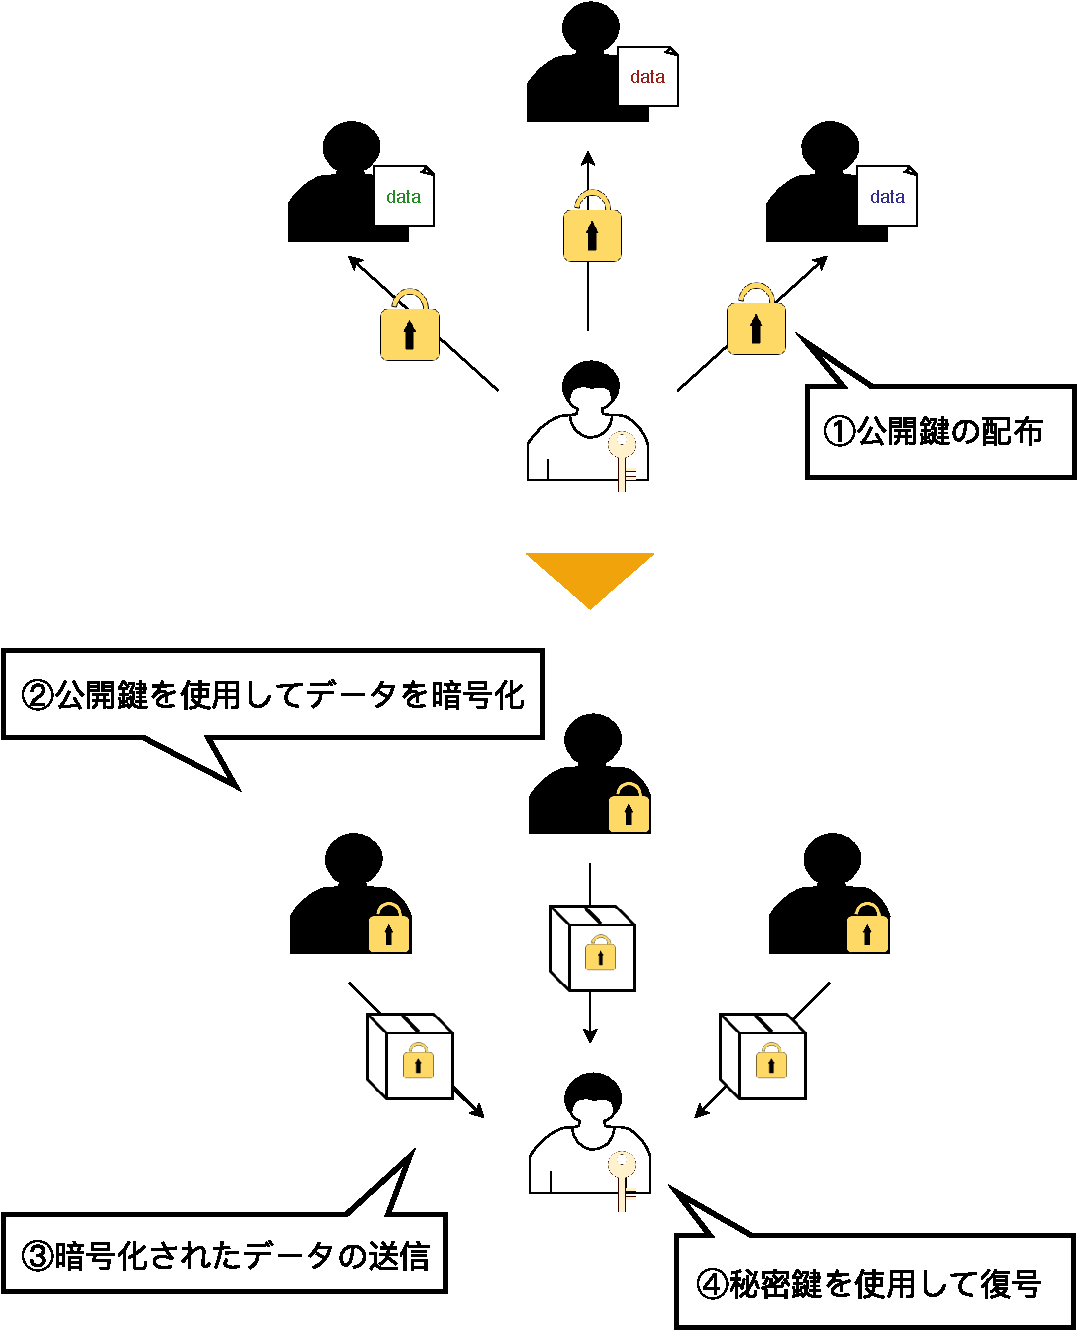
\includegraphics[width=10cm]{kokai.pdf}
\caption{公開鍵暗号通信の流れ}
\label{fig:no}
\end{figure} 

公開鍵暗号は共通鍵暗号とは違い各ユーザーごとに鍵を生成する必要がない.
また鍵の受け渡しの際に傍受される可能性がある共通鍵暗号通信とは違い,公開鍵では復号することができない.そのため共通鍵暗号通信よりも安全性が高い.しかし復号に複雑な計算を用いるため負荷が大きくなるため通信に時間がかかるという欠点もある.



\subsubsection{RSA暗号}
RSA暗号とは現在インターネットで広く使われている公開鍵暗号の一つである.
発明者であるRonald Linn Rivest,Adi Shamir,Leonard Max Adlemanの頭文字をとって名付けられた.
RSA暗号は桁数の多い素数の掛け算をするのは簡単だが,その合成数の素因数分解をするのは困難であることを安全性の根拠としている.


\subsubsection{電子署名の仕組み}

RSA暗号や楕円曲線DSAなど電子署名の役割を持つ暗号方式もある.
これらの公開鍵と秘密鍵が同じ構造をしている暗号では,どちらの鍵を使っても暗号化することができる.
そのため秘密鍵で暗号化し,公開鍵で復号することによって,送信者が本人であることを確認することができる.

\begin{figure}[H]
\centering
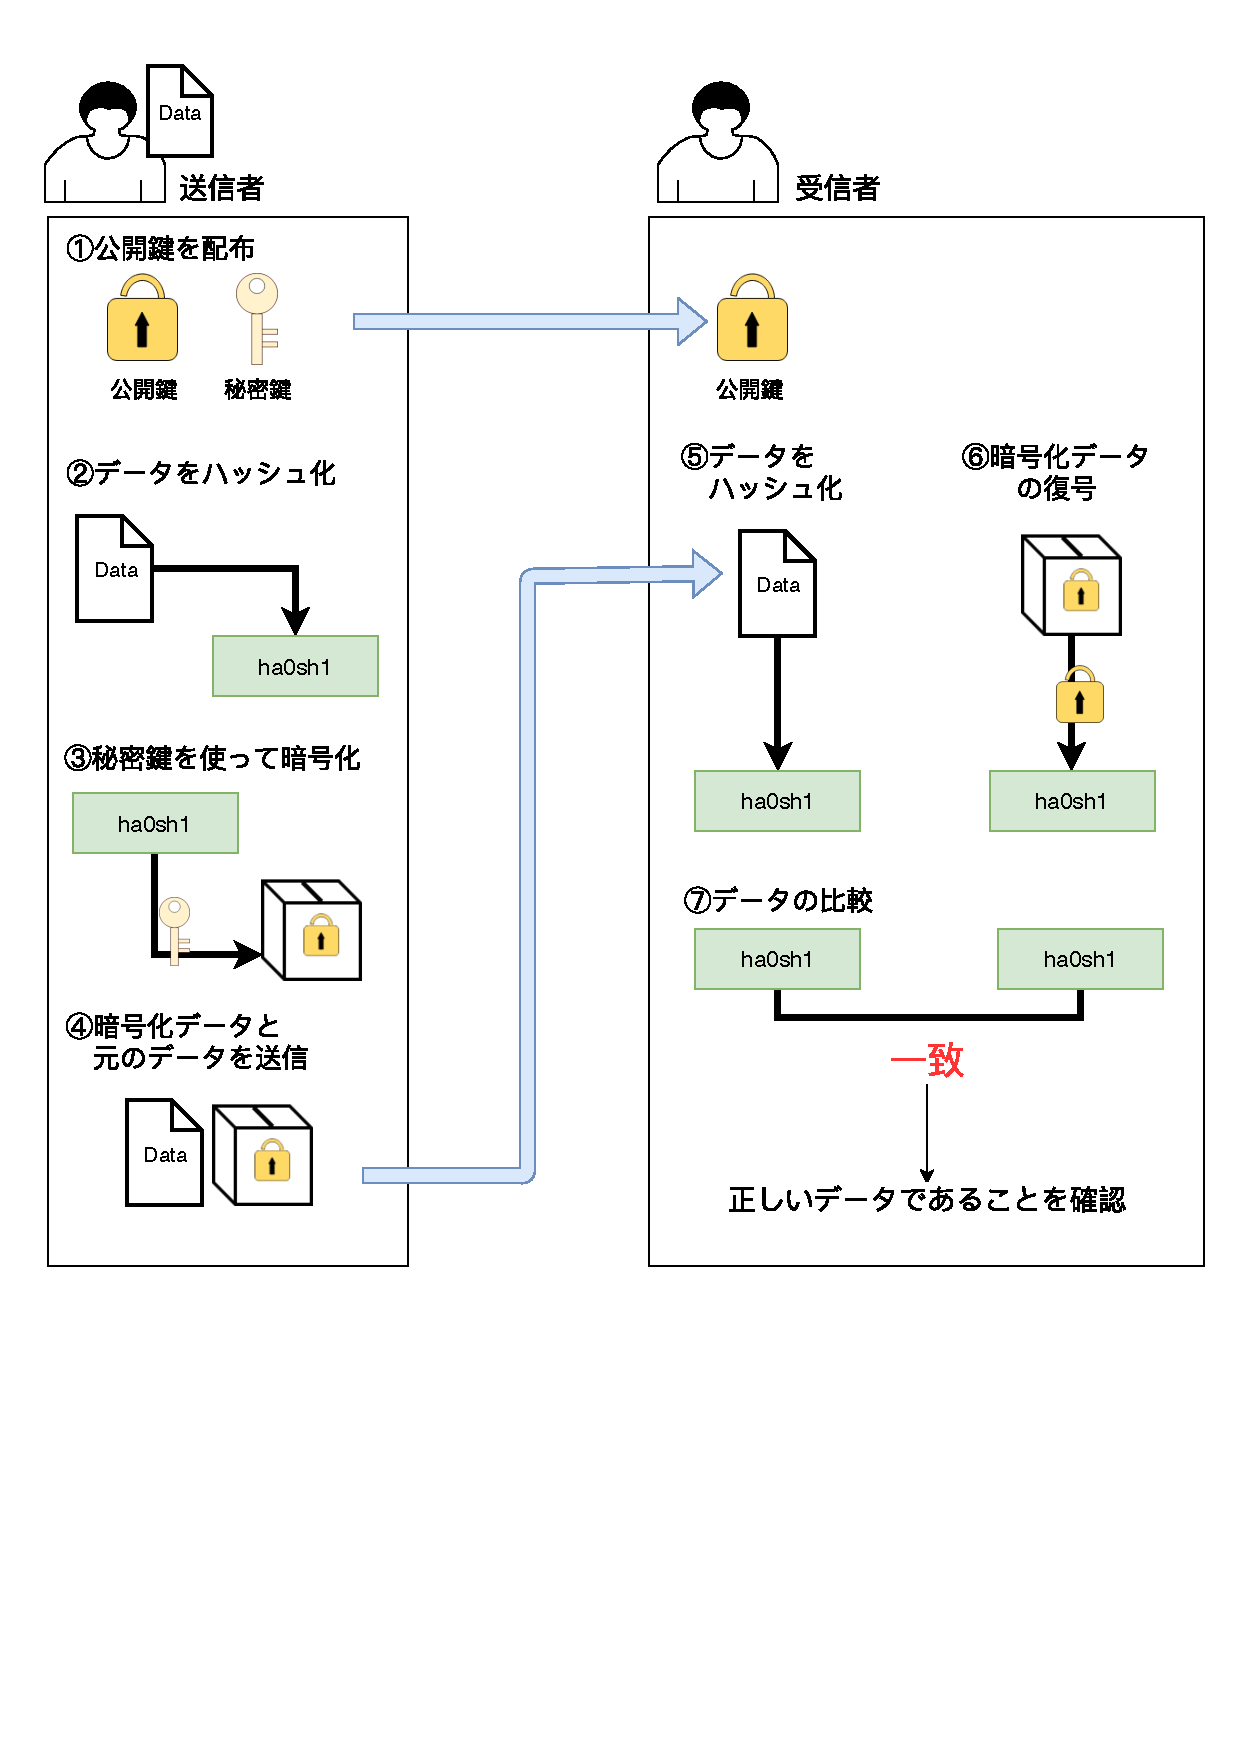
\includegraphics[mediaboxonly=/CropBox,width=12cm]{shomei.pdf}
\caption{電子署名の流れ}
\label{fig:no}
\end{figure} 





\subsection{SSL暗号化通信}
共通鍵暗号方式は公開鍵暗号方式よりも負荷が小さいが,鍵の受け渡し時に傍受される危険性があった.
そこで鍵の受け渡し時に公開鍵暗号方式を用いることで安全性を確保したものがSSL暗号化通信である.

\subsubsection{SSL暗号化通信の仕組み}

SSL暗号化通信では最初にユーザがサーバに接続要求を行い,送られてくるSSLサーバ証明書によって安全性を確認する.
安全性を確認したら,共通鍵を公開鍵暗号通信を使ってサーバに送ることで安全に共通鍵の受け渡しを行うことができる.




\begin{figure}[H]
\centering
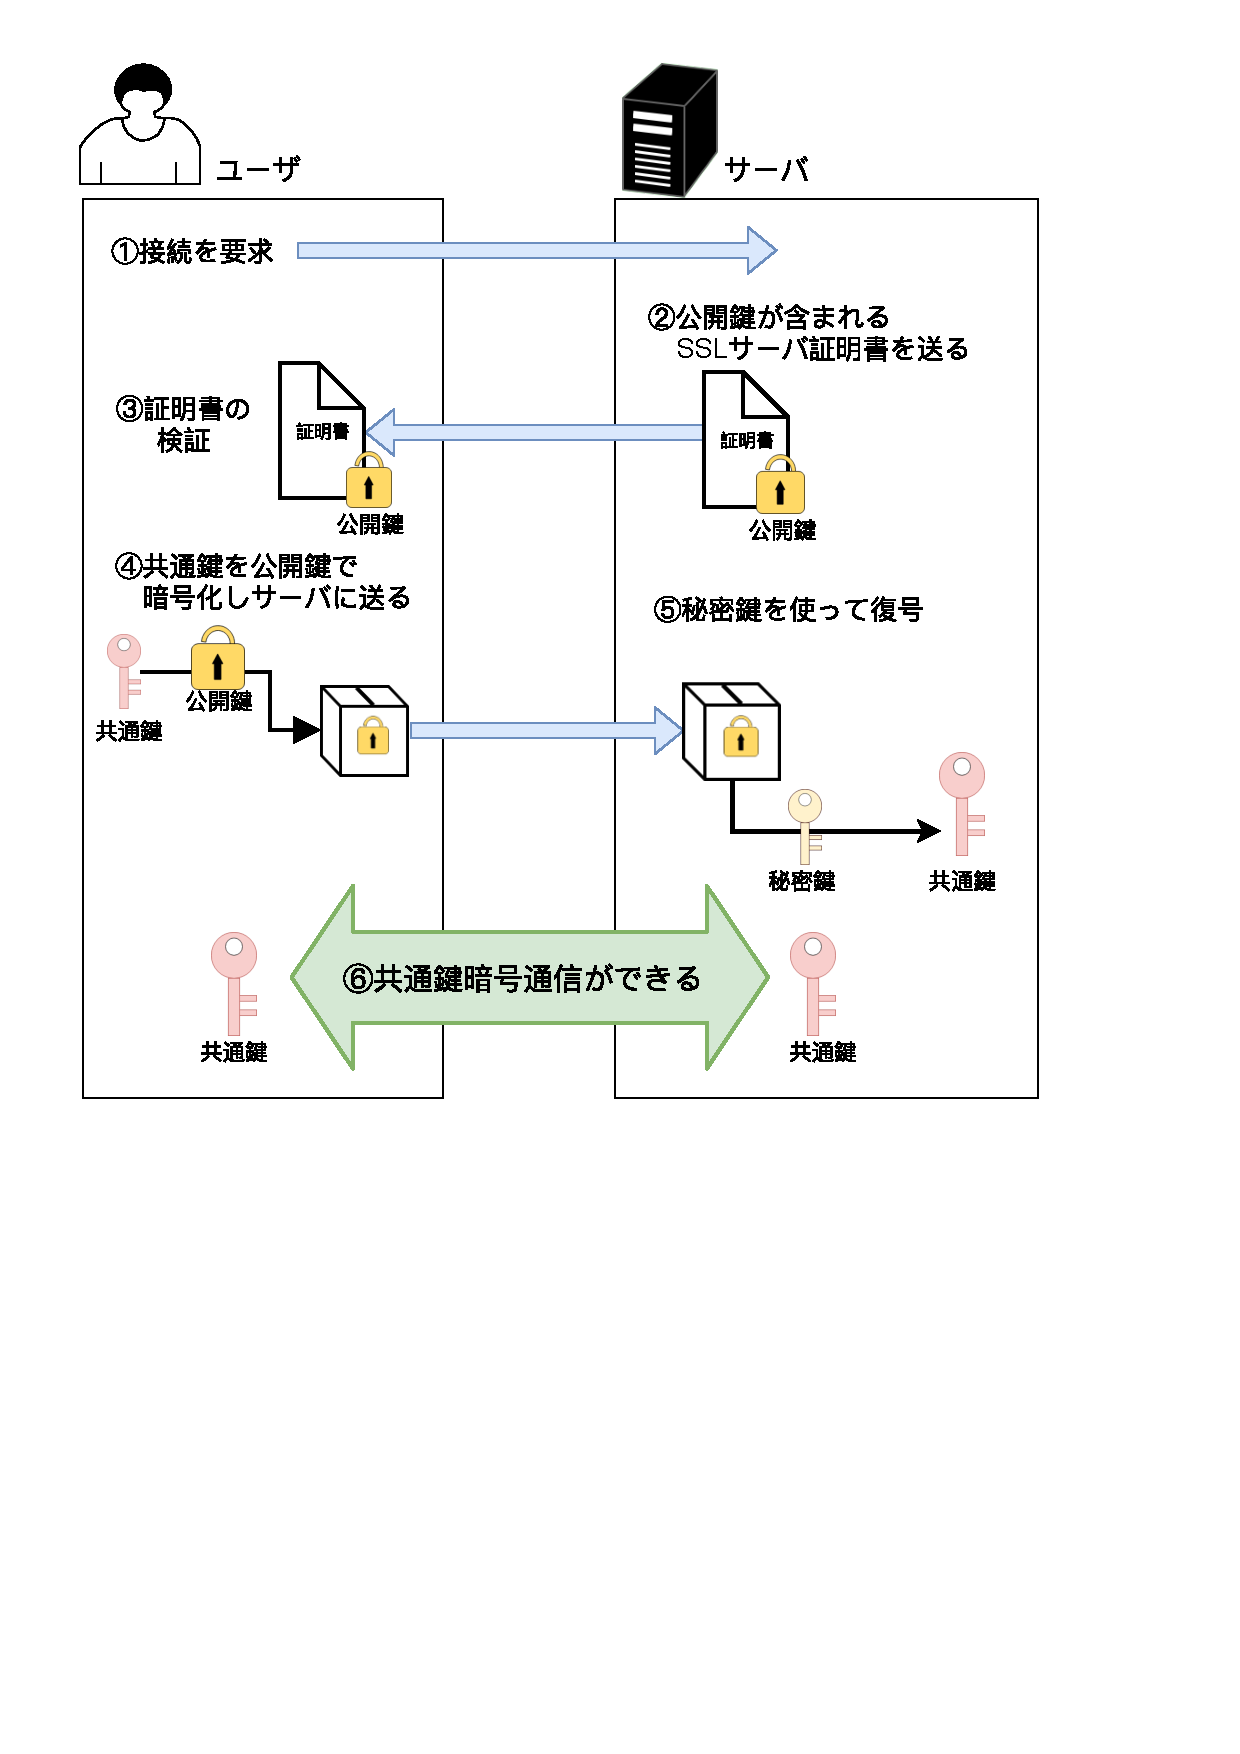
\includegraphics[mediaboxonly=/CropBox,width=14cm]{SSL.pdf}
\caption{SSL暗号化通信の流れ}
\label{fig:no}
\end{figure} 



\newpage
\section{ブロックチェーン}
ブロックチェーンとは,2009年にSatoshi Nakamoto氏の論文\cite{satoshi}で提唱された仮想通貨であるビットコインの根幹技術として生まれた分散型台帳システムである.


\subsection{ブロックチェーンの特徴}

取引を記録する台帳の1ページをブロックという.
ブロックチェーンはインターネット上の複数のコンピュータでお互いに取引の記録を共有し,検証しながら正しい記録の入ったブロックを鎖のように繋げていく.

\begin{figure}[H]
\centering
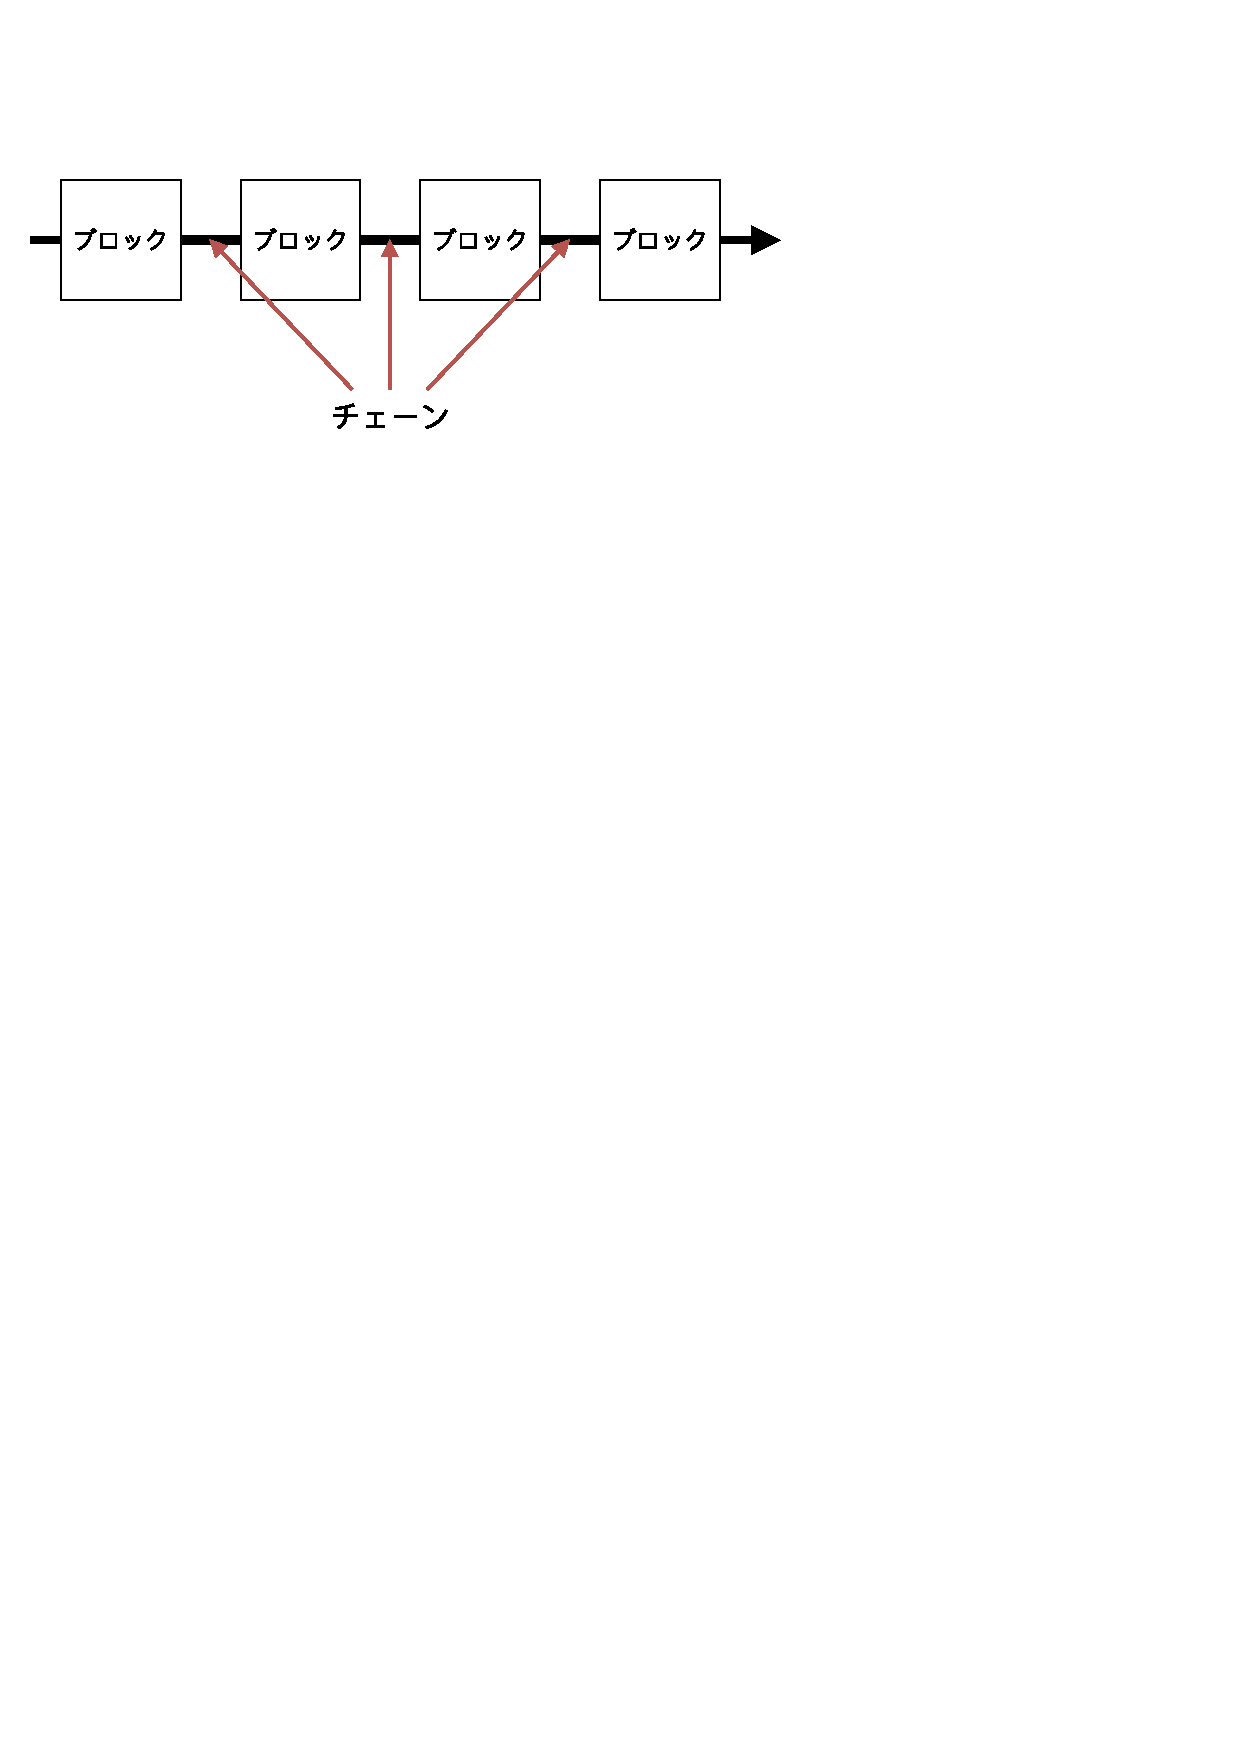
\includegraphics[mediaboxonly=/CropBox,width=11cm]{block1.pdf}
\caption{ブロックチェーンとは}
\label{fig:no}
\end{figure} 


\subsubsection{改ざんへの耐性がある}
ブロックチェーンの各ブロックはハッシュ関数によって繋がれている.ハッシュは不可逆性を持っており,ハッシュ値から元のデータを復元することはできない.ブロックチェーンでは複数の取引データがハッシュ化によって1ブロックにまとめられ,次のブロックに追加される.そのため過去のブロックを改ざんすると次のブロックとの整合性が取れなくなるため改ざんが困難である.


\newpage
\subsubsection{P2P分散型システム}
ブロックチェーンはP2P(Peer to Peer)を用いて取引データをやりとりしている分散型のシステムである.
P2Pは特定の管理者がサーバを管理するクライアント・サーバ型とは違い,各ノード間で対等に直接通信を行い,ネットワークを形成するネットワークである.
\begin{figure}[H]
\centering
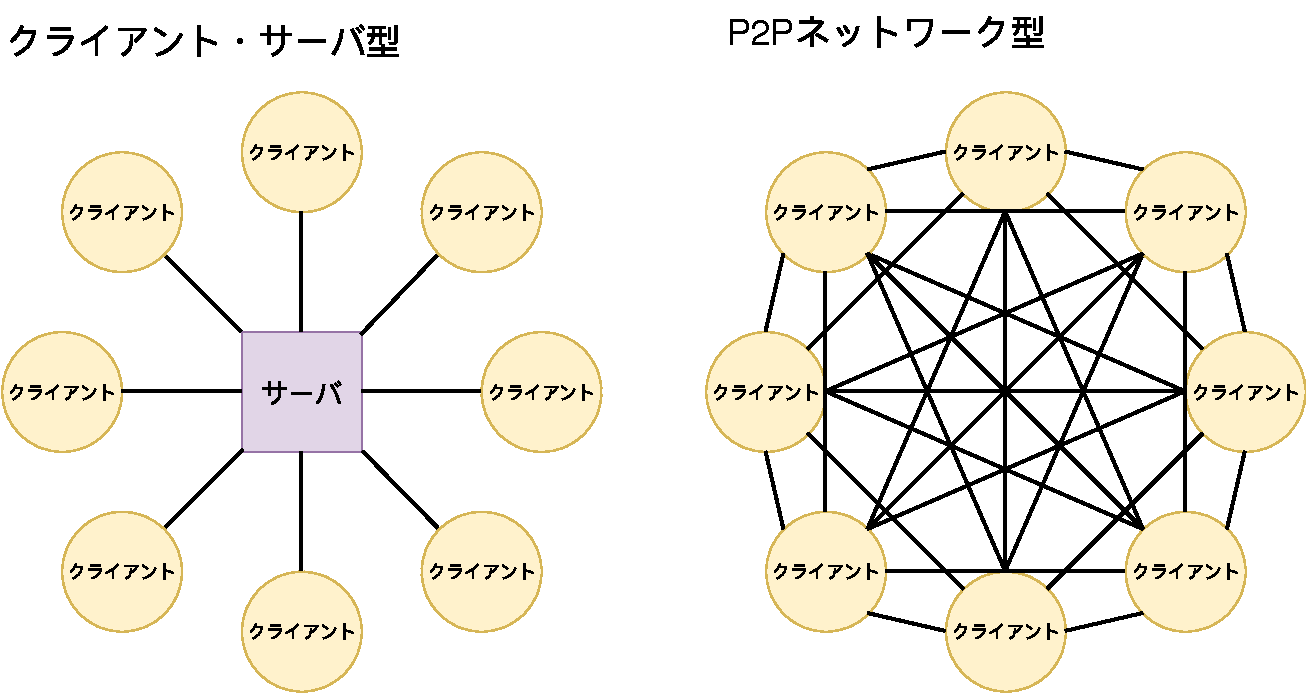
\includegraphics[width=13cm]{P2P.pdf}
\caption{クライアント・サーバ型とP2Pネットワーク型の違い}
\label{fig:no}
\end{figure} 



ブロックチェーンはP2Pネットワーク型であるため,データをまとめて記録したり,管理をしている機関のない非中央集権的なシステムとなっている.そのため一部のコンピュータに障害が発生してもシステムを維持することができる.

\subsubsection{ユーザとブロックチェーン間での通信}
ユーザとブロックチェーン間での通信には公開鍵暗号とハッシュを用いた電子署名の技術が使われる.
取引記録をハッシュ化したものを取引記録と一緒にブロックチェーンに送ることで,取引をしたユーザが本人であることを確認している.




\subsubsection{コンセンサスアルゴリズム}
チェーンにブロックを追加するにあたって,参加しているノードによる承認手続が必要となる.
ブロックチェーンでは管理者がいないため「不正」か「正当」の振り分けを,参加しているノードがある一定の条件のもとで行っている.またその一定の条件を満たしたノードが新たなブロックを作成する.

\subsection{仮想通貨とは}
一般的にはネットワーク上で電子的な決済の手段として流通しているが,法定通貨のように特定の国家による裏付けのないものである.ただし様々な種類の仮想通貨があり,定義や分類などは一様ではない.




\newpage
\subsection{コンセンサスアルゴリズムによるブロックチェーンの分類}
\subsubsection{Proof of Work(PoW)}
PoWではネットワークに参加しているノードは一番最初にnonceと呼ばれる値に当てはまる解を探す.このnonceを探す作業を採掘(マイニング)と呼ぶ.
採掘に成功したノードはブロックを作成し,ブロックチェーンをつなげる権利を得ることができる.

ビットコインではこのPoW方式が採用されている.
ビットコインの採掘では報酬として計算量に応じたビットコインをもらうことができる.\\

PoWの問題点としては総計算能力の過半数を占めるノードを用いることで虚偽のブロックを有効にすることができる51%問題がある.またPoWで報酬を得るためには高性能のコンピュータを常に起動して計算作業をさせる必要があり,無駄に電気コストがかかるという欠点もある.\\

\subsubsection{Proof of Stake(PoS)}
PoSでもブロック追加のためにはハッシュ関数等の計算による解が必要となるが,PoWでは計算量に応じた報酬を与えていたのに対し,仮想通貨の保有量に応じた報酬が与えられる.これはPoWの採掘に対し,鋳造(minting, forge)と呼ばれる.

またPoSではPoWと違い,計算量で争うことがなくなるため,PoWに比べ必要な電気コストが大幅に減らすことができる\cite{shu}.

PoWで51%攻撃をするためには膨大な計算能力を保有する必要があったが,PoSでは仮想通貨の総発行枚数の51%以上を保有する必要があり,PoWよりもコストがかかる.また自分が多く保有している通貨に攻撃を仕掛けるため,攻撃者にとってはメリットがあまりない.\\


しかしPoSでは通貨を保有することで報酬がもらえるという仕組みのため,通貨に必要な流動性が低くなってしまうという問題や流動性が低くなることで,仮想通貨の価格が低いときに大量に保有した人に報酬が集まり,貧富の差が広がるという問題がある.

\subsubsection{Proof of Importance(PoI)}

PoIでは参加者の重要度によって発言権が付与される.重要度は仮想通貨の保有量と取引(仮想通貨の流動性を高めたか)によって決められる.
PoSでは富裕層が有利になるというデメリットがあったが,PoI方式では流動性が高まるため,貧富の差が極端に広がることがない.PoIの仕組みによって報酬を得ることをハーベスティング(収穫)と呼ぶ.\\

しかしハーベスティングに参加するためには一定量の仮想通貨を保有する必要があり,PoSほどではないが富裕層が力を持つのではないかという懸念がある.



\newpage
\subsection{Proof of Workにおけるブロックチェーンの仕組み}
\subsubsection{ブロックに含まれるデータ}
ブロックにはハッシュ化した前の取引データの入ったブロック,取引データ,nonceが入っている.

\begin{figure}[H]
\centering
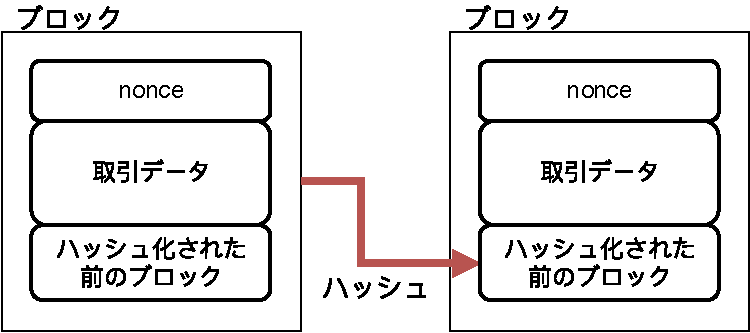
\includegraphics[width=11cm]{block2.pdf}
\caption{ブロックに含まれるデータ}
\label{fig:no}
\end{figure} 


\subsubsection{nonceの計算}
nonceは一定の長さの任意の値である.
nonceに数字を入れていき,ハッシュ化されたブロックの頭に0が一定数続くときにnonceを確定する.

ハッシュの元データは復元することができないため,nonceは総当たり的に探していくことになる.

\begin{figure}[H]
\centering
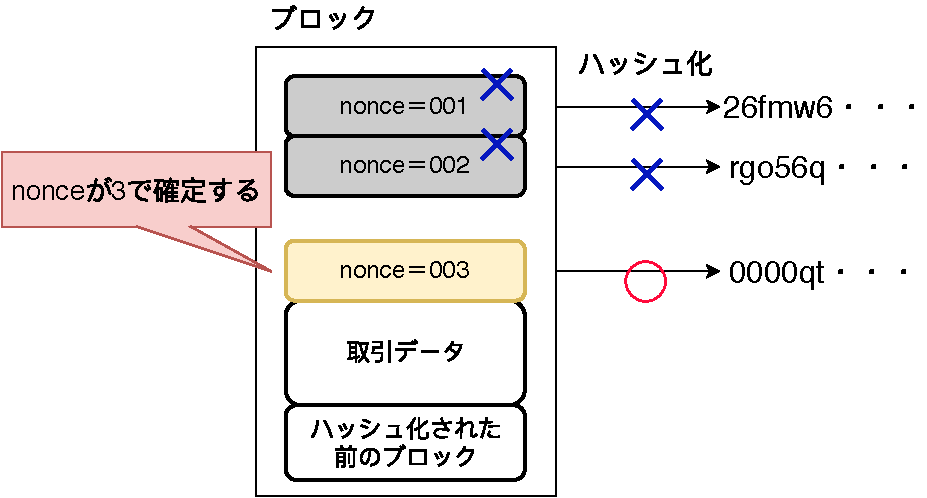
\includegraphics[width=14cm]{nonce.pdf}
\caption{nonceの計算}
\label{fig:no}
\end{figure} 

そのためデータが改ざんされると,改ざんされたブロック以降のnonceを全て総当たり的に探し直すこととなるためブロックチェーンが短くなる.ブロックチェーンが分岐したときは最も長いブロックチェーンのみを有効とするというルールがあるため,昔のブロックの改ざんほど難しくなる.

\begin{figure}[H]
\centering
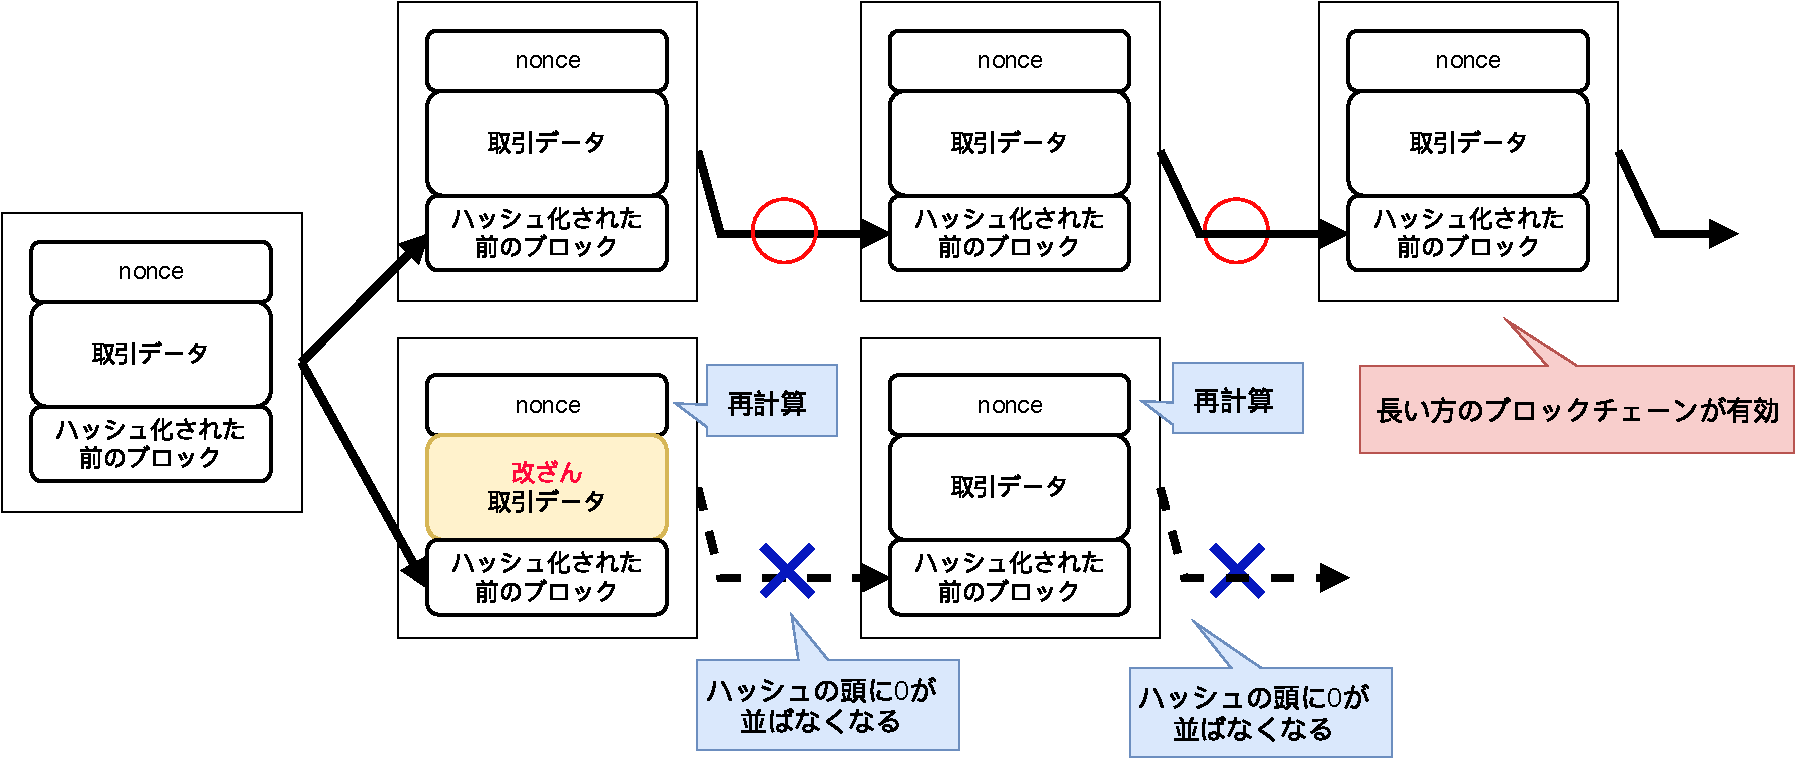
\includegraphics[width=14cm]{blockk.pdf}
\caption{改ざんを防ぐ仕組み}
\label{fig:no}
\end{figure} 

\newpage
\section{本研究で提案する仮説}
まず国際学力調査などで低得点を取る学生は特定の箇所が苦手なのではなく,「どこがわかっていないのかもわからない」「そもそもいま何を教えられているかもわからない」など根本的な理由で勉強ができていないと考えた.
その原因を問題を解くことが目的となっており,学習した知識を日常生活に結びつけることができていないことや,また結びつけることを推奨するような教育カリキュラムになっていないと考えた.
そこで問題を解くことを目的にするのではなく,その技術を使って何ができるかを意識させることが,学力の向上につながると考えている.


図\ref{fig:03}に表した通り,積み上げ型教科には3通りある.
その中でも複数の単元を前提知識として用いる単元を学習する際には以下の問題があると考えた.

\begin{itemize}
\item 学習の目的がわかりづらい\\
主に数学などでは,計算方法を学習した後にそれを使った技術などを学習することが多いように感じられた.
この仮説を用いることによって,その技術で必要な答えが何かを明確にできると考えた.
また,学習のイメージがしやいことや,学習に対するモチベーションの向上などにもつながると考えた.

\item どの単元の知識を使えばいいかがわかりづらい\\
複数の前提知識となる単元を用いることで,学習内容がどちらの単元のものであったかなど混乱する学生がいると考えた.
\end{itemize}


そこで前提知識を複数用いる単元をあらかじめ学習し,全体の流れを理解することで,前提知識となる単元の理解の促進につながると考えた.



\newpage
\section{実験}
本章では,提案した仮説が正しいことを証明するために実験を行う.以下で実験方法の解説を行う.
\subsection{実験目的}
本研究で提案した「学習する単元を前提知識とする単元の概要をあらかじめ理解することで,内容の理解を促進することができる」という仮説が正しいことを証明することを目的とする.

\subsection{実験方法}
\subsubsection{実験期間}

情報数学応用の講義にて3週かけて行う.

1週目:平成30年11月16日

2週目:平成30年11月30日

3週目:平成30年12月7日


\subsubsection{実験方法}

Aクラスでは仮説を用いない講義を行い,Bクラスでは仮説を用いた講義を行う.最後に両クラスで同一の小テストを行い,点数の比較と分析を行う.
また小テストと同じ用紙にて比較対象を同条件にするためのアンケートを行う.

(1)講義スケジュール

実験を行う講義は図\ref{fig:timeline}のように行う.
仮説を用いないAクラスでは最初に暗号とハッシュについて学習した後に,ブロックチェーンについて学習する.
仮説を用いたBクラスでは最初に暗号とハッシュを前提知識とするブロックチェーンの概要について学習した後に,暗号とは負について学習する.

\begin{figure}[H]
\centering
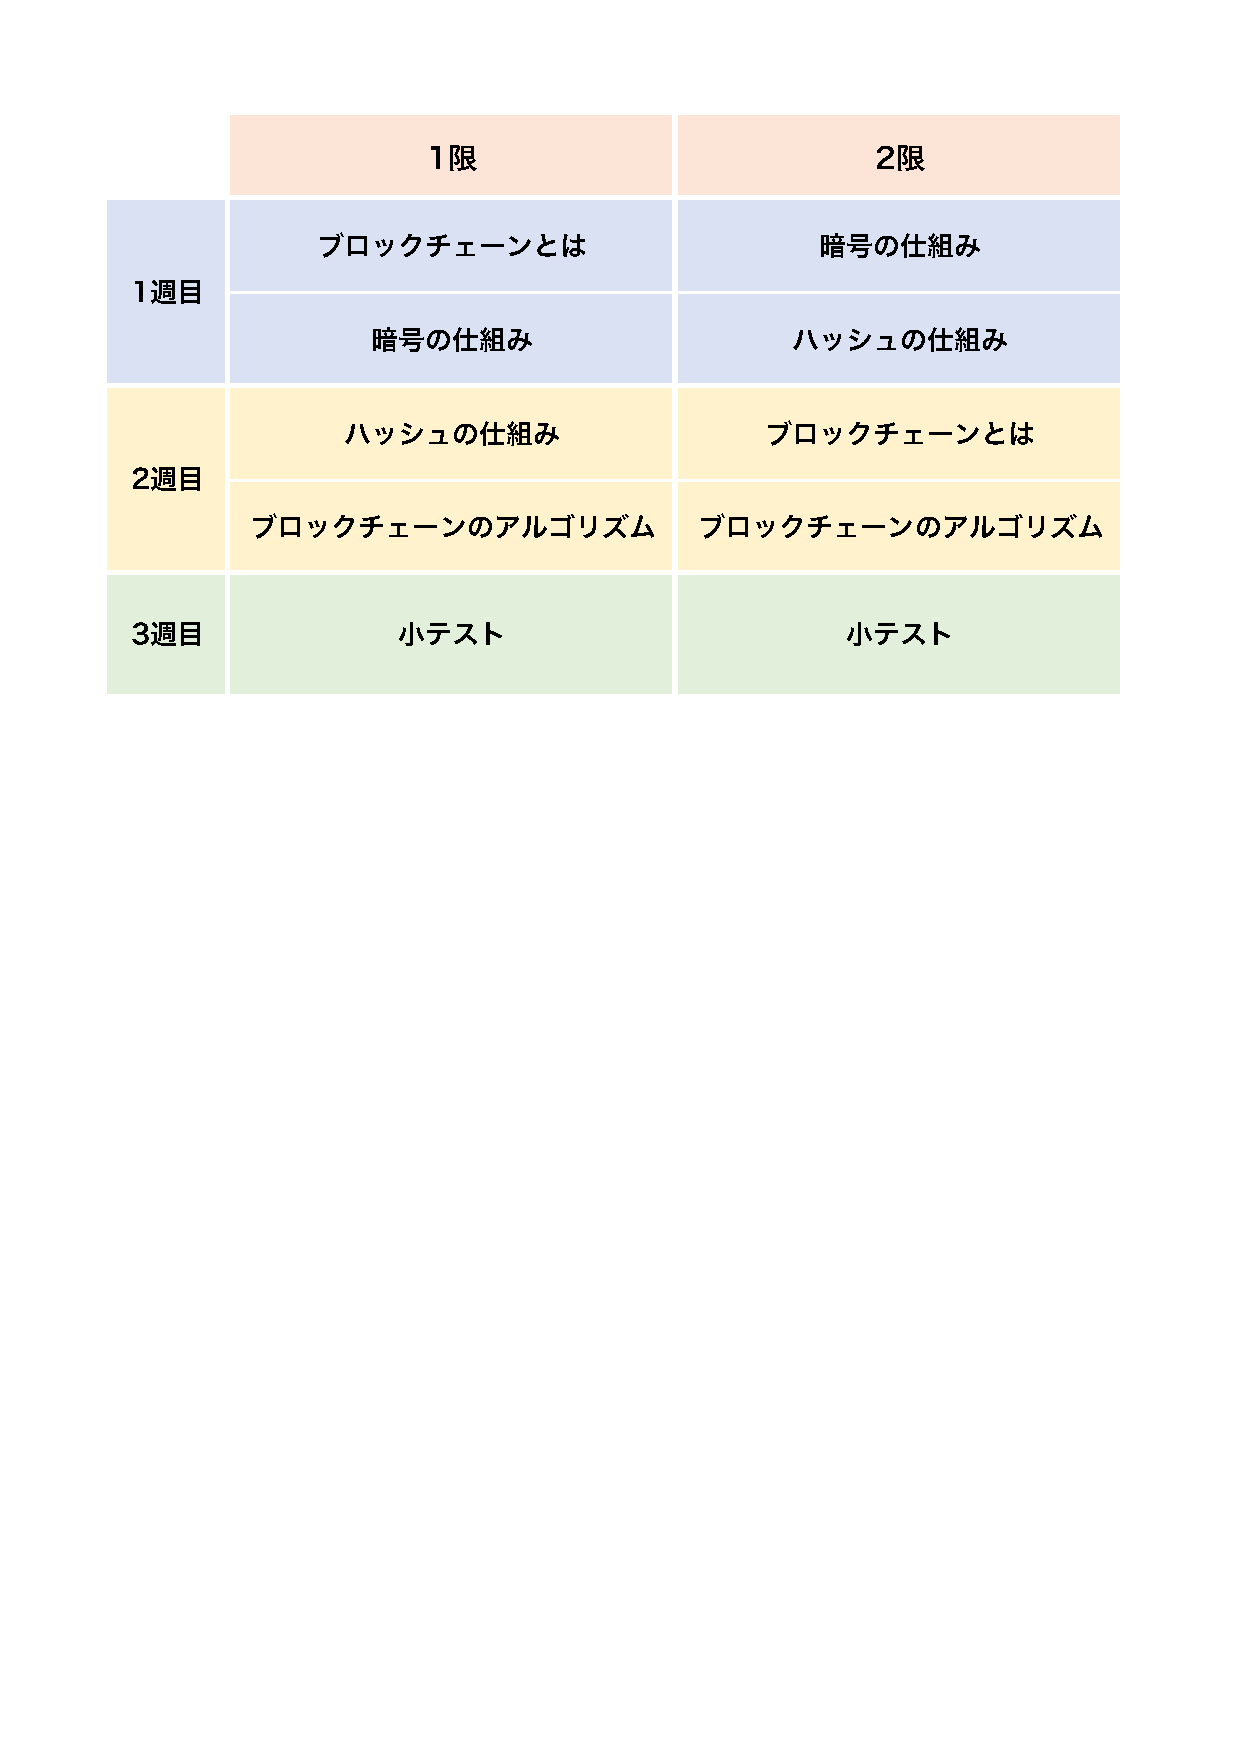
\includegraphics[mediaboxonly=/CropBox,width=12cm]{timeline.pdf}
\caption{講義スケジュール}
\label{fig:timeline}
\end{figure} 

(2)アンケートについて

アンケートにて「ブロックチェーンについて講義を受ける前に学習したことがあるか」について「はい」「いいえ」の二択で聞いた.
「はい」と答えた学生は仮説の「あらかじめ内容を理解する」に該当するが,人数に偏りができることと,元の知識により高得点を取る可能性が高いことから,比較の対象とはせず参考程度に留める.

またアンケート未回答の学生も比較の対象としないこととする.
\\


(3)小テスト内容

小テストでは以下の内容を問う.

\UTF{2460}RSA暗号の特徴

\UTF{2461}ハッシュと暗号の違い

\UTF{2462}ブロックチェーンの仕組み

点数配分は\UTF{2460}+\UTF{2461}で5点,\UTF{2462}で5点の合計10点とする.\\


(4)評価方法について

「前提知識となる単元」「前提知識を用いた単元」「合計」の3つの観点で点数を比較する.
「前提知識となる単元」は \UTF{2460}RSA暗号の特徴 \UTF{2461}ハッシュと暗号の違い,「前提知識を用いた単元」は \UTF{2462}ブロックチェーンの仕組み,「合計」は小テスト全体の点数(\UTF{2460}+\UTF{2461}+\UTF{2462})について平均点と点数の分布を比較する.
また元の学力の差を考慮して,中間試験の満点を今回の実験で行う小テストに合わせ,平均点の差を比較する.

\subsubsection{実験対象}

千葉工業大学 情報科学部 情報ネットワーク学科の学生のうち

2018年後期に開講された情報数学応用の受講者

Aクラス76名,Bクラス76名,計152名とする.\\

ただし複数回の講義を用いての実験であるため,比較や分析に使用するデータは小テスト受験者のみである.
またアンケートの結果,受講前にブロックチェーンを学習してことがない学生で,中間試験を受験している学生を比較と分析の対象とする.





\newpage
\section{実験結果}
\subsection{アンケート結果と分析対象者}
各クラスのアンケートの結果は表\ref{fig:ank}のようになった.\\


\begin{table}[H]
\centering
\scalebox{1.2}{
\begin{tabular}{|c|c|c|}
\hline
\multicolumn{1}{|l|}{} & \multicolumn{1}{l|}{Aクラス} & \multicolumn{1}{l|}{Bクラス} \\ \hline
学習したことがない              & 60                      & 56                      \\ \hline
学習したことがある              & 4                       & 4                       \\ \hline
アンケート未回答               & 3                      & 2                       \\ \hline
小テスト未受験                & 9                      & 14                       \\ \hline
\end{tabular}
}
\caption{アンケート結果}
\label{fig:ank}
\end{table}

またブロックチェーンを学習したことがない学生のうち,中間試験を受験した学生は\ref{fig:ank2}の通りとなった.

\begin{table}[H]
\centering
\scalebox{1.2}{
\begin{tabular}{|c|c|c|}
\hline
\multicolumn{1}{|l|}{} & \multicolumn{1}{l|}{Aクラス} & \multicolumn{1}{l|}{Bクラス} \\ \hline
受験した             & 59                      & 54                      \\ \hline
未受験              & 1                       & 2                       \\ \hline
\end{tabular}
}
\caption{中間試験の受験状況}
\label{fig:ank2}
\end{table}

この結果より小テストの点数の比較はAクラスが59人,Bクラスが54人の計113人で行う.

\subsection{中間試験の平均点と点数換算}
中間試験は50点満点であるため,小テストとの比較のために5点満点と10点満点に換算する.


\begin{table}[H]
\centering
\scalebox{1.2}{
\begin{tabular}{|c|c|c|}
\hline
\multicolumn{1}{|l|}{} & \multicolumn{1}{l|}{Aクラス} & \multicolumn{1}{l|}{Bクラス} \\ \hline
50点満点      & 29.37         &  28.00                                         \\ \hline
5点満点    & 2.94      & 2.80                                              \\ \hline
10点満点      & 5.87       & 5.60                                            \\ \hline
\end{tabular}
}
\caption{中間試験の受験状況}
\label{fig:ank2}
\end{table}



\newpage
\subsection{小テストの点数}
\subsubsection{前提知識となる単元}
\UTF{2460}RSA暗号の特徴 \UTF{2461}ハッシュと暗号の違い の点数分布と平均点は以下のようになった.

\begin{figure}[H]
\centering
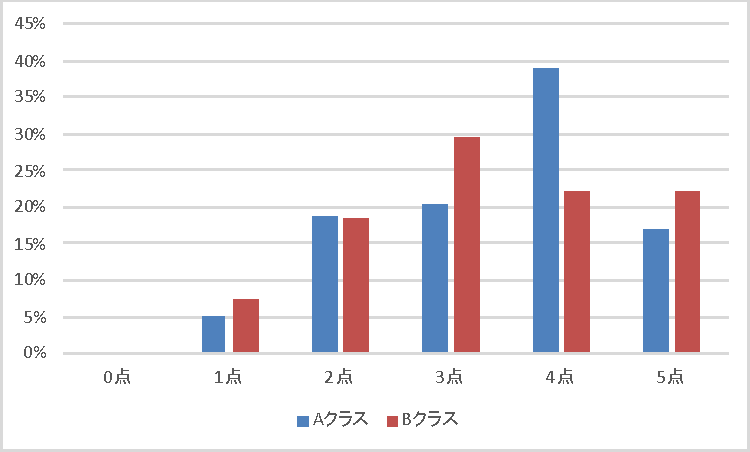
\includegraphics[width=12cm]{12test.pdf}
\caption{前提知識となる単元の点数分布}
\label{fig:no}
\end{figure} 

\begin{table}[H]
\centering
\scalebox{1.2}{
\begin{tabular}{|c|c|c|}
\hline
\multicolumn{1}{|l|}{} & \multicolumn{1}{l|}{Aクラス} & \multicolumn{1}{l|}{Bクラス} \\ \hline
中間試験                                    & 2.94       & 2.80               \\ \hline
小テスト                                  & 3.44       & 3.33                 \\ \hline
小テスト-中間試験                    & 0.50          & 0.53                           \\ \hline
\end{tabular}
}
\caption{前提知識となる単元の平均点の比較}
\label{fig:12ank}
\end{table}

平均点は仮説を用いていないAクラスの方がわずかに高くなったが,中間試験の点数と比較したところほとんど差は見られなかった.

\newpage
\subsubsection{前提知識を用いた単元}
\UTF{2462}ブロックチェーンの仕組み の点数分布と平均点は以下のようになった.

\begin{figure}[H]
\centering
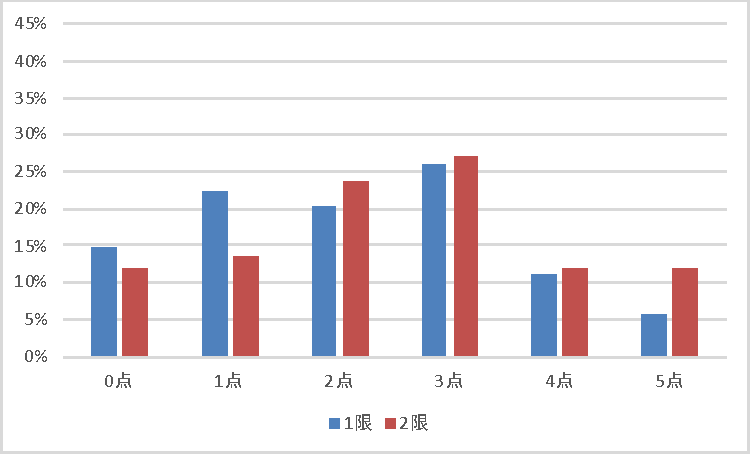
\includegraphics[width=12cm]{3test.pdf}
\caption{前提知識を用いた単元の点数分布}
\label{fig:no}
\end{figure} 


\begin{table}[H]
\centering
\scalebox{1.2}{
\begin{tabular}{|c|c|c|}
\hline
\multicolumn{1}{|l|}{} & \multicolumn{1}{l|}{Aクラス} & \multicolumn{1}{l|}{Bクラス} \\ \hline
中間試験                   & 2.94       & 2.80                                \\ \hline
小テスト                       & 2.49       & 2.13                           \\ \hline
小テスト-中間試験                           & -0.45            & -0.67                  \\ \hline
\end{tabular}
}
\caption{前提知識を用いた単元の平均点の比較}
\label{fig:12ank}
\end{table}

平均点,中間試験との差のどちらもAクラスの方がわずかに高くなるという結果となった.




\newpage
\subsubsection{小テスト全体}

\begin{figure}[H]
\centering
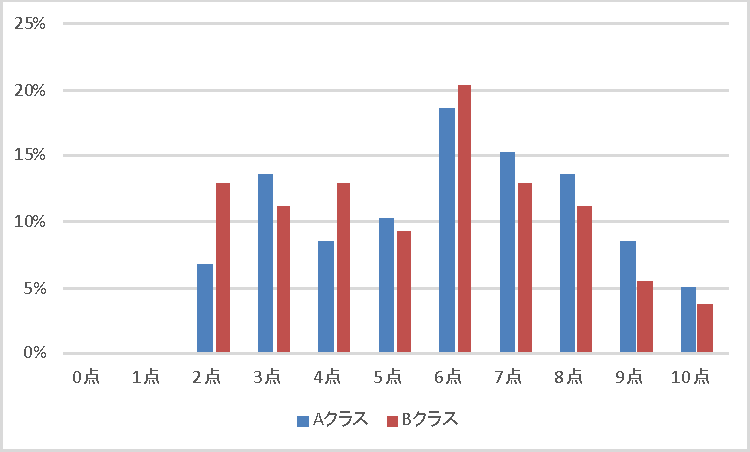
\includegraphics[width=12cm]{123test.pdf}
\caption{小テスト全体の点数分布}
\label{fig:no}
\end{figure}

\begin{table}[H]
\centering
\scalebox{1.2}{
\begin{tabular}{|c|c|c|}
\hline
\multicolumn{1}{|l|}{} & \multicolumn{1}{l|}{Aクラス} & \multicolumn{1}{l|}{Bクラス} \\ \hline
中間試験              & 5.87      & 5.60                                    \\ \hline
小テスト                        & 5.93        & 5.46                         \\ \hline
小テスト-中間試験                    & 0.06       & -0.14                             \\ \hline
\end{tabular}
}
\caption{小テスト全体の平均点の比較}
\label{fig:12ank}
\end{table}

5点以上はどちらのクラスにおいても同じような得点分布の形となった.5点未満は仮説を用いたBクラスの人数が多くなっている.
 


\newpage
\section{考察}
今回の実験では仮説を証明することができなかった.
そこで「実験方法」「仮説」の二つの観点から原因を考察した.

\subsection{実験方法}
\subsubsection{スケジュール}
まず今回の実験は講義の時間にて行った.図\ref{fig:timeline}で示した通り,講義と試験の間でテスト勉強をする時間があったため,講義のみでの理解度が測ることができなかった可能性がある.
また講義と小テストを別日で行ったため講義を欠席して小テストのみ受けた学生などの考慮が甘く,講義と小テストを受けた学生のみで実験を行うべきであった.

また祝日を跨いでしまった

\subsubsection{試験問題}

図\ref{fig:test5}で示すように「前提知識となる単元」「前提知識を用いた単元」の問題の難易度に差ができてしまった.簡単な問題は講義から時間が経っていても解けるが,難解な問題は内容を忘れやすく,時間が経っているクラスの点数に影響が出ている可能性がある.

\begin{table}[H]
\centering
\scalebox{1.1}{
\begin{tabular}{|c|c|c|}
\hline
\multicolumn{1}{|l|}{} & \multicolumn{1}{l|}{Aクラス} & \multicolumn{1}{l|}{Bクラス} \\ \hline
前提知識となる単元                       & 3.44      & 3.33                           \\ \hline
前提知識を用いた単元                           & 2.49      & 2.13                        \\ \hline
\end{tabular}
}
\caption{前提知識を用いた単元の平均点の比較}
\label{fig:test5}
\end{table}

\subsubsection{授業の選定}
今回の実験で前提知識として扱った暗号やハッシュには他の講義で扱った行列や誤り検出訂正などの前提知識が必要である.元の学力の差を考慮するために中間試験の点数との比較を行ったが,本実験に関係する知識の元の学力を測るものとは言えなかったため点数にズレが生じてしまった可能性がある.

また仮説を提唱した理由の一つが「前提知識となる単元の目的をはっきりさせることで理解が促進できる」ことであったが,今回の実験で用いた暗号技術やハッシュは実用例が割と身近にあり,ブロックチェーンを目的にするよりもわかりやすいと感じる学生が多かったかもしれない.

\newpage
\subsection{仮説}
今回の仮説において「先にブロックチェーンを学習しても内容が全く理解できずに講義についていけなくなる」ということが1番の懸念点であった.小テストのブロックチェーンの問題で仮説を使用したクラスの点数が悪くなっていることからこの懸念通り,ブロックチェーンが理解が浅くなってしまったと考えた.

そのため今回の仮説では積み上げ型教科という広い範囲での仮説を立てたが,細かい条件を考えることで一部の講義では仮説が利用できる可能性がある.

\newpage
\section{結言}
文部科学省が発表した国際学力調査によると世界の中でも日本の学力は上位にある.しかし日本よりも上位の国に比べ.低得点の割合はやや多く,順位を上げるためには低得点層の割合を減らすことが必要である.
低得点層の学生は学習内容の一部がわからないのではなく,「何をしているのかがわからない」「どこがわからないのかもわからない」などという根本的な原因があると推測している.

また各塾の調査では中学,高校で学習する科目の中で数学と英語は苦手になりやすいと言われている.この2科目の共通点である積み上げ型教科という点に注目した.積み上げ型教科とは既に学習した知識を使うことを前提として授業を行う教科である.そのため単元の内容が複雑になるほど必要な前提知識が多くなり,どの単元の内容が使われているかがわかりにくくなる.そのためその単元の内容を理解をすることが難しくなることが問題点としてあげられる.

そこで本研究では積み上げ型教科での理解力向上を目的として,「学習する単元を前提知識とする単元の概要をあらかじめ説明することで,内容の理解を促進することができる」という仮説を立て,仮説の証明を目指した.
しかし今回行った実験のみでは仮説が正しいことを証明することができなかった.しかし実験方法に多くの改善点が見つかったため,仮説が間違っていると断定することもできないという結果になった.



\newpage
\section{参考文献}
\begin{thebibliography}{9}
\bibitem{1}
ベネッセ教育情報サイト:“教科学習が不得意と感じている高校生が9割!そのほとんどが英語と数学に偏るのにはある理由が”, \url{https://www.benesse.jp/kyouiku/201603/20160329-3.html}, (参照 2018-8-14)
\bibitem{satoshi}
Satoshi Nakamoto, “Bitcoin:A Peer-to-Peer Electronic Cash System”,2009年
\bibitem{shu}
 ”コンセンサスアルゴリズムとは?「PoW・PoS・PoI」の種類と違いを解説”.はじめてのビットコイン.\url{https://www.newscrypto.jp/articles/2612},(参照 2019-1-9)
\end{thebibliography}

\section{謝辞}
本研究の遂行および本論文の作成にあたり,多くの御助言と御指導いただきました須田宇宙准教授に深く感謝の意を表します.
また実験に協力していただいた情報数学応用の受講者に深く感謝の意を表します.

\section{付録}

\end{document}
